\chapter{Experimentos}

\label{ch:experiments}

\section{Introducción}

La idea principal detrás del perfil de experimentación propuesto en este trabajo es la de poder demostrar que las características neurofisiológicas incorporadas en este modelo computacional son relevantes para dotar al mismo con capacidades de adquisición y posterior clasificación fonética robusta e invariante. Las cualidades fonéticas dinámicas son extraídas por el modelo de manera completamente no supervisada, adquiriendo la estadística espectro-temporal inmersa en las cualidades fonotácticas de los estímulos. Las capacidades de invarianza y generalización fonéticas del modelo son evaluadas merced a su competencia a la hora de entrenar un algoritmo de clasificación supervisado como el \gls{svm}. Estimamos que el desempeño de clasificación fonética del \gls{svm} frente a versiones distorsionadas en las respuestas del modelo ante diferentes perturbaciones ambientales--como el ruido blanco y la reverberación--o las corridas de tono, constituye un indicador claro de las propiedades existentes en las características espectro-temporales del modelo.

\section{Clasificación Fonética, un Caso de Estudio}

Proponemos un modelo computacional llamado \gls{cstm}, que consiste de dos partes: El \gls{el} y el \gls{mrstsa}.  

%We propose a computational approach called \gls{cstm}, which consists of two parts: The \gls{el} and the \gls{mrstsa}.  

EL algoritmo \gls{mrstsa}, el cual procesa las ondas de sonido para alimentar la entrada al \gls{el}, es una técnica inspirada en Chi T. et al. \cite{chi_2005}. En su trabajo, hallazgos experimentales acumulados desde el sistema auditivo central se explotaron demostrando su aplicación en la evaluación objetiva de la inteligibilidad del habla. En el presente trabajo, debido a que promovemos la incorporación parsimoniosa de propiedades neurofisiológicas--principalmente centradas en las características de la corteza--seguimos las líneas principales en la implementación de la sección cortical de tal modelo.

%The algorithm \gls{mrstsa}, which processes the sound waves to feed inputs to the \gls{el}, is a technique inspired by Chi T. et al. \cite{chi_2005}. In their work, accumulating experimental findings from the central auditory system were exploited demonstrating its applications in the objective evaluation of speech intelligibility. In the present work, since we prompt a parsimonious incorporation of neurophysiological properties--mainly centered in cortical features--we followed the main guidelines in the implementation of the cortical section of such model.

El \gls{el} convierte un arreglo multidimensional de números reales en un \gls{sdr} multidimensional. Esta etapa está compuesta por un conjunto de \glspl{som} \cite{kohonen_2082, Kohonen:1989:SAM:69371} e incorpora fenómenos neurofisiológicos como la organización columnar, la formación aferente espontánea micro-columnar, las arborizaciones dendríticas próximas y distantes, la interacción intercolumnar lateral por medio de activaciones de ramas dendríticas independientes con receptores \gls{nmda}, los \glspl{mfe} con adaptación a estímulos contextuales, inhibición intracolumnar lateral próxima, \gls{ltp}, \gls{ltd}, \gls{stdp} y regulaciones homeostáticas sináptica.

%The \gls{el} converts a multidimensional array of real numbers into a multidimensional \gls{sdr}. This stage is composed by a set of \glspl{som} \cite{kohonen_2082, Kohonen:1989:SAM:69371} and incorporates neurophysiological phenomena such as columnar organization, afferent spontaneous micro-columnar formation, proximal and distal dendritic arborization, lateral intercolumn interaction by means of independent dendritic \gls{nmda} branch activations, \glspl{mfe} with contextual stimulus adaptation, proximal lateral intracolumn inhibition, \gls{ltp}, \gls{ltd}, \gls{stdp} and distal synaptic homeostatic regulations.

En el presente trabajo, estudiamos el nivel de invarianza en las características fonéticas abstraídas por el \gls{el}, por medio de la comparación de tales representaciones con características auditivas espectro-temporales de múltiple resolución devueltas por el algoritmo \gls{mrstsa}. A tal efecto, evaluamos las características devueltas por cada algoritmo en diferentes tareas de clasificación de palabras. Para probar el desempeño en clasificación de palabras en cada algoritmo, utilizamos la técnica \gls{svm} con la configuración experimental delineada en la Fig. \ref{fig:Experiment}.

%In the present work, we studied the level of invariance in the phonetic features abstracted by the \gls{el}, by means of comparing such representations with the multiresolution spectro-temporal auditory features returned by the \gls{mrstsa} algorithm. To this end, we evaluated the features returned by each algorithm in different word classification tasks. In order to asses the word classification performance in each algorithm, we used \gls{svm} technique with the experimental setup depicted in Fig. \ref{fig:Experiment}.

\begin{figure}[h!]
    \centering
    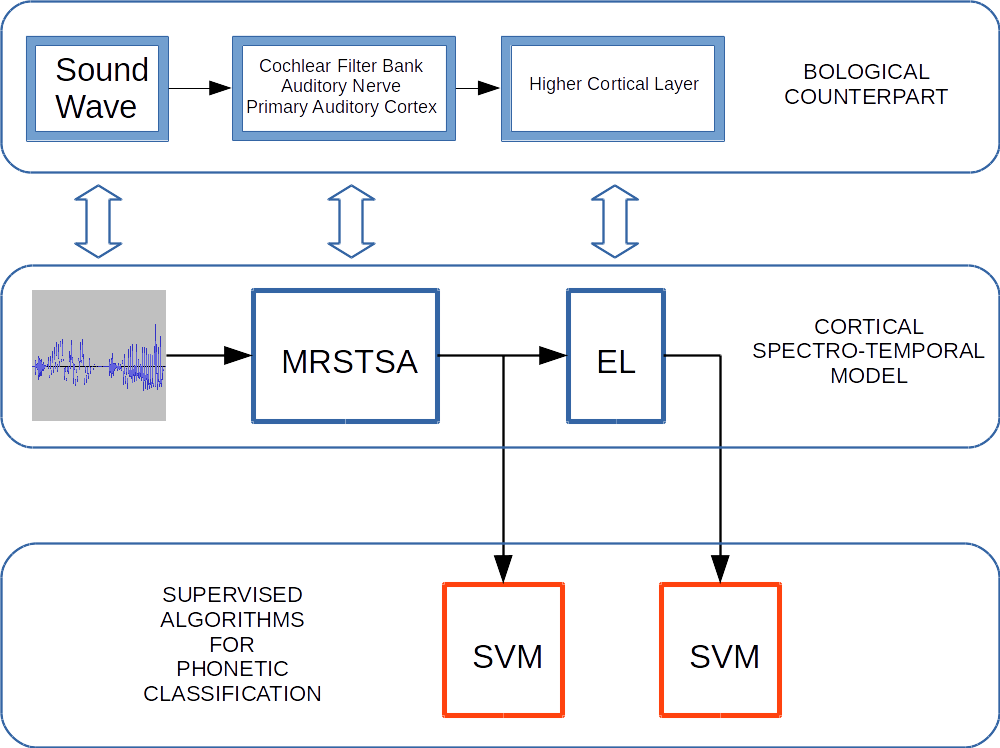
\includegraphics[width=0.7\textwidth]{Experiment.png}
    \caption{Configuración experimental para probar el desempeño en las tareas de clasificación de palabras. Las ondas de sonido son procesadas por el algoritmo \gls{mrstsa}. Las salidas desde el \gls{mrstsa} son procesadas por el \gls{el}. Las tareas de clasificación de palabras son realizadas sobre ambas salidas por medio del algoritmo \gls{svm}. Cada sección en el \gls{cstm} tiene su contrapartida biológica.}
    %\caption{Experimental setup to test word classification task performances.
    %Sound waves are processed by the \gls{mrstsa} algorithm.
    %The outputs from the \gls{mrstsa} are processed by the \gls{el}.
    %Word classification tasks are performed on both outputs by the \gls{svm} algorithm.
    %Each section in the \gls{cstm} has its biological counterpart.}
    \label{fig:Experiment}
\end{figure}

\pagebreak

En el procedimiento experimental primero entrenamos el \gls{el} con un corpus original de 500 palabras desde un vocabulario de 5 palabras con 10 voces diferentes (8 masculinas y 2 femeninas) generadas por el sintetizador de habla \gls{festival} \cite{festival2014}. Luego, procesamos el mismo corpus con el \gls{el} en modo de inferencia. En tal modo, el \gls{el} procesa la información con las propiedades de aprendizaje deshabilitadas. De esta manera, durante la inferencia, el \gls{el} no modificó sus sinapsis y sólo devolvió patrones de activación en respuesta a los estímulos que recibió. Luego utilizamos las salidas desde el \gls{mrstsa} y desde el \gls{el} en modo de inferencia para entrenar los clasificadores \gls{svm}. El desempeño de los entrenamientos con validación cruzada se muestra en la Tabla \ref{SVM_Training}.

%In the experimental procedure we first trained the \gls{el} with an original corpus of 500 words from a vocabulary of 5 words with 10 different voices (8 males and 2 females) generated by \gls{festival} Synthesis \cite{festival2014} speech synthesizer. Afterwards, we processed the same corpus with the \gls{el} in inference mode. In such mode, the \gls{el} processed the information with its learning properties disabled. In this manner, during inference, the \gls{el} did not modify its synapses and just returned patterns of activation in response to the stimuli it received. We then used the outputs from the \gls{mrstsa} and the \gls{el} in inference mode to train the \gls{svm} classifiers. The cross validation training performances are shown in Table~\ref{SVM_Training}.

\begin{table}[h!]
\centering
\caption{Resultados para el entrenamiento del \gls{svm} con validación cruzada de 5-secciones (5-fold cross validation training results)}
\begin{tabular}{|l|l|l|}
\hline
		   & MRSTSA & Encoder Layer \\ \hline
Monosyllabic Words & 98.8\% & 99\%          \\ \hline
Disyllabic Words   & 98\%   & 97.8\%        \\ \hline
Trisyllabic Words  & 97.6\% & 98\%          \\ \hline
\end{tabular}
\label{SVM_Training}
\end{table}

\pagebreak

En una segunda etapa, corrimos el \gls{el} en modelo de inferencia nuevamente, pero esta vez afectamos el corpus original por medio de diferentes tipos de varianzas. Testeamos el desempeño del los clasificadores ya entrenados en presencia de las características devueltas por los algoritmos en repuesta a los corpus afectados por las varianzas introducidas a los corpus originales por medio de Audacity \cite{audacity}. Las varianzas introducidas incluyeron ruido blanco, reverberación y variaciones de tono. 

%In a second stage, we ran the \gls{el} in inference mode again, but this time we affected the original corpus by means of different kind of variances. We tested the performances of the--already trained--classifiers in the presence of the features returned by the algorithms in response to the corpus affected by the variances which we introduced to original corpora by means of Audacity \cite{audacity}. The variances introduced to the original corpus included white noise, reverberation and pitch variations. 

\section{Resultados}

Los desempeños de clasificación se muestran en las Figs. \ref{fig:MONO_ACC}, \ref{fig:DI_ACC} and \ref{fig:TRI_ACC}.

%The classification performances are shown in Figs. \ref{fig:MONO_ACC}, \ref{fig:DI_ACC} and \ref{fig:TRI_ACC}.

\begin{figure}[h!]
    \centering
    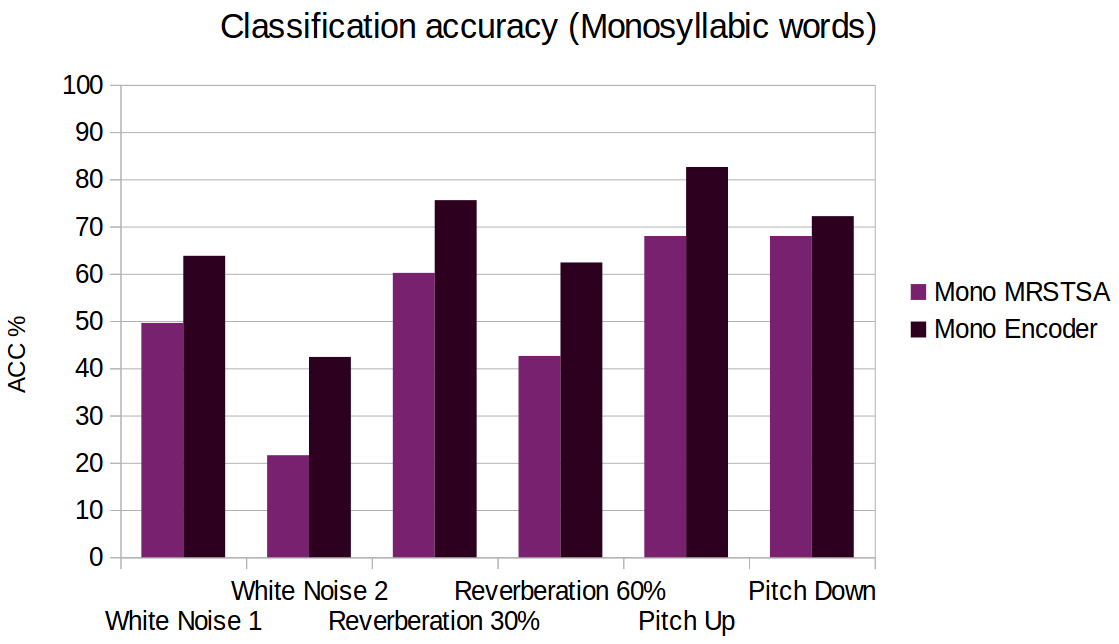
\includegraphics[width=0.9\textwidth]{MONO_ACC.png}
    \caption{Precisión en la clasificación realizada sobre el \gls{mrstsa} y el \gls{el} contra diferentes varianzas introducidas en las señales originales
    para \textbf{palabras monosilábicas}.
    White Noise 1 determina una relación de señal a ruido o \gls{snr} tasa promedio de potencia \gls{rms} de 19.8 dB mientras que White Noise 2 13.8 dB.
    Reverberation 30\% determina un valor de \gls{rt} de 0.61 segundos mientras que Reverberation 60\% determina un valor de \gls{rt} de 1.78 segundos.
    Pitch Up determina un cambio de tono desde E a G, mientras que Pitch Down determina un movimiento de tono desde E a C.}
    %\caption{\gls{mrstsa} and \gls{el} classification accuracies against different variances introduced to the original signals
    %for \textbf{monosyllabic words}.
    %White Noise 1 determines a \gls{snr} average \gls{rms} power rate of 19.8 dB while White Noise 2 13.8 dB.
    %Reverberation 30\% determines a \gls{rt} value of 0.61 seconds while Reverberation 60\% determines a \gls{rt} value of 1.78 seconds.
    %Pitch Up determines a pitch move from E to G, while Pitch Down determines a pitch move from E to C.}
    \label{fig:MONO_ACC}
\end{figure}

\begin{figure}[h!]
    \centering
    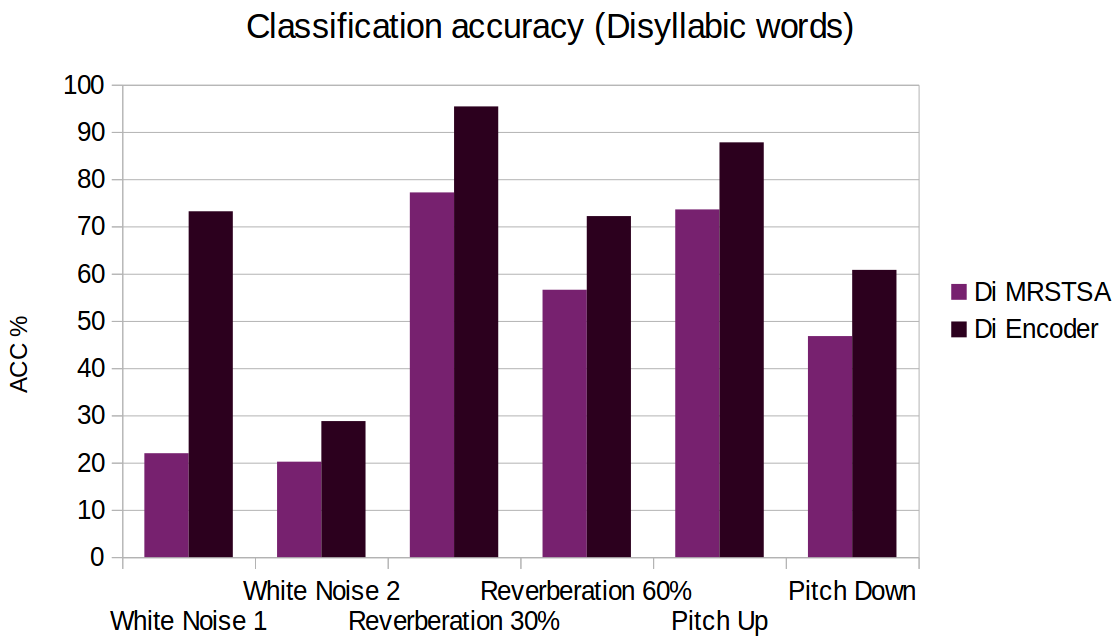
\includegraphics[width=0.9\textwidth]{DI_ACC.png}
    \caption{Precisión en la clasificación realizada sobre el \gls{mrstsa} y el \gls{el} contra diferentes varianzas introducidas en las señales originales
    para \textbf{palabras disilábicas}.
    White Noise 1 determina una relación de señal a ruido o \gls{snr} tasa promedio de potencia \gls{rms} de 19.8 dB mientras que White Noise 2 13.8 dB.
    Reverberation 30\% determina un valor de \gls{rt} de 0.61 segundos mientras que Reverberation 60\% determina un valor de \gls{rt} de 1.78 segundos.
    Pitch Up determina un cambio de tono desde E a G, mientras que Pitch Down determina un movimiento de tono desde E a C.}
    %\caption{\gls{mrstsa} and \gls{el} classification accuracies against different variances introduced to the original signals
    %for \textbf{disyllabic words}.
    %White Noise 1 determines a \gls{snr} average \gls{rms} power rate of 19.8 dB while White Noise 2 13.8 dB.
    %Reverberation 30\% determines a \gls{rt} value of 0.61 seconds while Reverberation 60\% determines a \gls{rt} value of 1.78 seconds.
    %Pitch Up determines a pitch move from E to G, while Pitch Down determines a pitch move from E to C.}
    \label{fig:DI_ACC}
\end{figure}

\begin{figure}[h!]
    \centering
    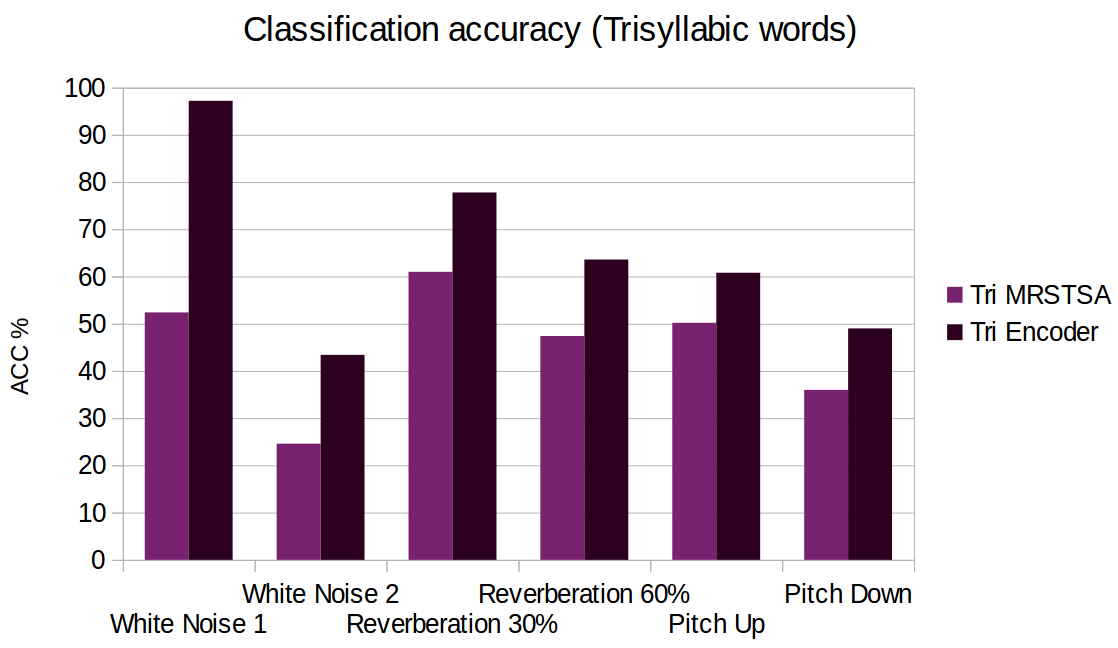
\includegraphics[width=0.9\textwidth]{TRI_ACC.png}
    \caption{Precisión en la clasificación realizada sobre el \gls{mrstsa} y el \gls{el} contra diferentes varianzas introducidas en las señales originales
    para \textbf{palabras trisilábicas}.
    White Noise 1 determina una relación de señal a ruido o \gls{snr} tasa promedio de potencia \gls{rms} de 19.8 dB mientras que White Noise 2 13.8 dB.
    Reverberation 30\% determina un valor de \gls{rt} de 0.61 segundos mientras que Reverberation 60\% determina un valor de \gls{rt} de 1.78 segundos.
    Pitch Up determina un cambio de tono desde E a G, mientras que Pitch Down determina un movimiento de tono desde E a C.}
    %\caption{\gls{mrstsa} and \gls{el} classification accuracies against different variances introduced to the original signals
    %for \textbf{trisyllabic words}.
    %White Noise 1 determines a \gls{snr} average \gls{rms} power rate of 19.8 dB while White Noise 2 13.8 dB.
    %Reverberation 30\% determines a \gls{rt} value of 0.61 seconds while Reverberation 60\% determines a \gls{rt} value of 1.78 seconds.
    %Pitch Up determines a pitch move from E to G, while Pitch Down determines a pitch move from E to C.}
    \label{fig:TRI_ACC}
\end{figure}

\pagebreak

En relación con el ruido blanco, introducimos ruido blanco aditivo a la señal original con una tasa de potencia de señal a ruido promedio o \gls{rms} de 19.9 dB (White Noise 1) y 13.8 dB (White Noise 2). En términos de reverberación, modificamos la señal original por medio de valores de \gls{rt} de 0.61 segundos (Reverberation 30\%) y 1.78 segundos (Reverberation 60\%). \gls{rt} es el tiempo que la señal toma para decrecer en su amplitud a 60 dBs por debajo de su valor inicial. En relación a las variaciones de tono, modificamos el tono de la señal en un +20\% (de E a G) (Pitch Up) y en --20\% (de E a C) (Pitch Down).

%Regarding white noise, we introduced additive white noise to the original signal with a signal-noise average \gls{rms} power rate of 19.9 dB (White Noise 1) and 13.8 dB (White Noise 2). In terms of reverberation, we modified the original signal by means of \gls{rt} values of 0.61 seconds (Reverberation 30\%) and 1.78 seconds (Reverberation 60\%). \gls{rt} Is the time that a signal takes to decrease its amplitude to 60 dBs under its initial value. As regards pitch variations, we modified the signal pitch in +20\% (from E to G) (Pitch Up) and in --20\% (from E to C) (Pitch Down).

Las Figs. \ref{fig:MONO_ACC}, \ref{fig:DI_ACC} y \ref{fig:TRI_ACC} muestran la exactitud en una tarea de clasificación de 5 vías para palabras mono, di y trisilábicas en los corpus afectadas por ruido blanco, reverberación y variaciones de tono. Como se puede ver en las figuras, el \gls{el} supera al \gls{mrstsa} en todos los casos. Tal comportamiento persiste para palabras multisilábicas.

%Figs. \ref{fig:MONO_ACC}, \ref{fig:DI_ACC} and \ref{fig:TRI_ACC} show a 5 way word classification accuracy for mono, di and trisyllabic word corpora affected by white noise, reverberation and pitch variations. As can be seen in the figures, the \gls{el} outperforms the \gls{mrstsa} in all cases. Such behavior persists for multisyllabic words.

La Fig. \ref{fig:AV_ACC} muestra la exactitud promedio en la clasificación a través de todas las varianzas para palabras mono, di y trisilábicas. Como se puede apreciar en la figura, de acuerdo con las barras de \textbf{Error Standard}, el encoder muestra con claridad una superioridad sustenida a través de palabras con diferentes números de sílabas.

%Fig. \ref{fig:AV_ACC} shows average classification accuracies across all variances for mono, di and trisyllabic words. As can be seen in the figure, according to \textbf{Standard Error} bars, the encoder layer clearly shows a sustained superiority across words with different number of syllables.

\begin{figure}[h!]
    \centering
    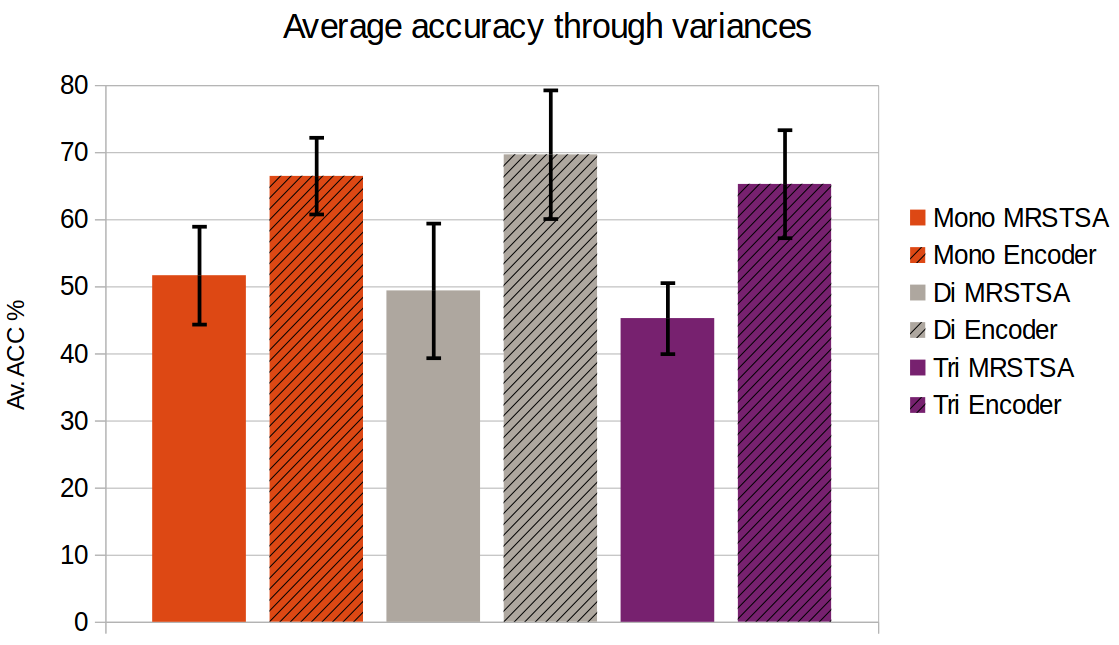
\includegraphics[width=0.9\textwidth]{AV_ACC.png}
    \caption{Promedio de exactitud en clasificación a través de todas las varianzas para palabras mono, di y trisilábicas con barras de Error Standard. Mono significa palabras monosilábicas, Di significa palabras disilábicas y Tri significa palabras trisilábicas.}
    %\caption{Average classification accuracies across all variances for mono, di and trisyllabic words with Standard Error bars.
    %Mono means monosyllabic words, Di means disyllabic words and Tri means trisyllabic words.}
    \label{fig:AV_ACC}
\end{figure}

\subsection{Barrido con \glspl{el} de diferentes tama\~nos}

Los \glspl{el} puestos bajo prueba para este trabajo tienen 15 por 15 (225) \glspl{cc}. Cada \gls{cc} cuenta con un arreglo de 15 por 15 (225) unidades neuronales. Por lo tanto los \glspl{el} probados en nuestros experimentos tienen un total de 50625 unidades neuronales contra una dimensionalidad de 5 por 128 (640) componentes desde el algoritmo \gls{mrstsa}. Aún cuando el funcionamiento del \gls{el} es completamente diferente al funcionamiento presentado por el algoritmo \gls{mrstsa}, el sustancialmente mayor número de dimensiones de salida del \gls{el} podría llevar a pensar que la mejora en el desempeño en clasificación fonética tiene sus orígenes en un simple aumento de la dimensionalidad y no en el cambio sustancial en la naturaleza secuencial del procesamiento de la información en el \gls{el}.

Por este motivo, decidimos correr pruebas con \glspl{el} de varios tama\~nos y observar el desempe\~no en clasificación fonética de cada uno de ellos. En la FIg \ref{fig:E_S} se muestran los parámetros de inicialización de los diferentes modelos. Se observa que el rango de \glspl{el} empieza con un modelo peque\~no de tan sólo una \gls{cc} con un campo receptivo lateral distante en ella misma hasta un \gls{el} con 21 por 21 (441) \glspl{cc} con un campo receptivo de 15 por 15 \glspl{cc} en torno a cada \gls{cc}.
\begin{figure}[h!]
    \centering
    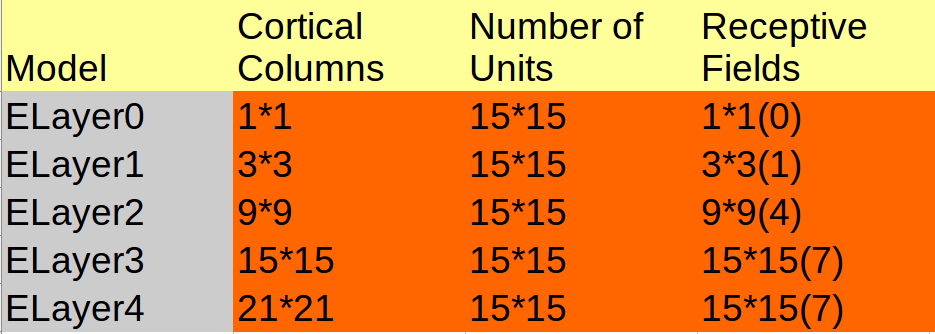
\includegraphics[width=0.6\textwidth]{Encoder_Swept.png}
    \caption{Diferentes \glspl{el} para realizar el barrido. En la primera columna de la tabla se tienen las dimensionalidades del \gls{el} en cuanto a las \glspl{cc}. En la segunda columna de la tabla se detalla la dimensionalidad de cada \gls{cc} en cuanto al número de unidades. Finalmente, en la tercera columna se detallan los campos receptivos laterales distantes de cada columna cortical. El número entre paréntesis junto a la especificación del campo receptivo es el parámetro con el que se debe inicializar dicho campo para obtener la dimensionalidad detallada. Por ejemplo, un campo receptivo de 3 por 3 indica que cada columna cortical puede vincularse con columnas corticales en un arreglo de 3 por 3 \glspl{cc} alrededor de la \gls{cc} en cuestión.}
    \label{fig:E_S}
\end{figure}

Como se puede apreciar en la FIg. \ref{fig:E_S1}, el desempe\~no de clasificación promedio es sustancialmente mayor para los \glspl{el}, aún para el \gls{el} número 0, el cual cuenta con tan solo 225 unidades neuronales, un número marcadamente inferior al número de dimensiones utilizadas por el algoritmo \gls{mrstsa}. Esto indica claramente que la mejora en el desempeño en clasificación fonética de palabras tiene un origen algorítmico más allá del aumento en la dimensionalidad de la salida. Por otro lado sí se observa una tendencia a mejorar el desempe\~no en clasificación promedio con \glspl{el} de mayor tama\~no. Esto puede deberse al aumento de la dimensionalidad presentada para los modelos con más unidades neuronales. Sin embargo pensamos que esto puede estar dado por un aumento en el número de dendritas distantes laterales y por consiguiente el aumento en la información predictiva en los \glspl{el} con más tama\~no. A través de visualizaciónes dinámicas hemos notado que el \gls{el} 0, incurre en una gran cantidad de \glspl{mfe}, lo cual indica una falta de información desde dendritas laterales para obtener \glspl{sdr}. Creemos que este podría ser uno de los motivos que explique el aumento en el desempe\~no en clasificación para modelos más grandes y no sólo el simple aumento en la dimensionalidad de la salida.


\begin{figure}[h!]
    \centering
    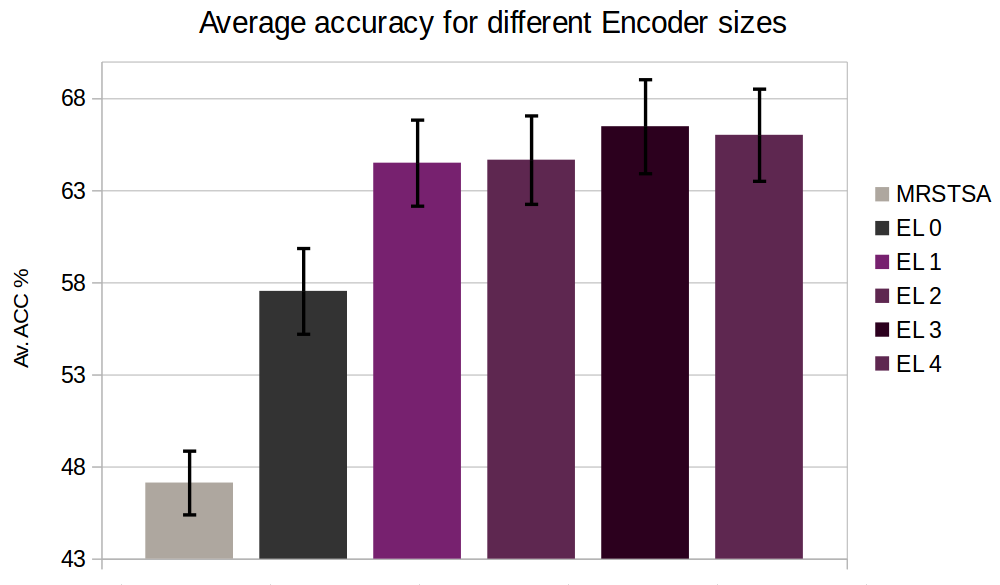
\includegraphics[width=0.9\textwidth]{Encoder_Swept1.png}
    \caption{Desempe\~no promedio de clasificación para los diferentes \glspl{el}. Para cada \gls{el} se computa el promedio de todas las pruebas de clasificación de palabras. Se debe tener en cuenta que dentro de este promedio se encuentran además, pruebas cruzadas de modelos entrenados con palabras monosilábicas y probados con palabras bisilábicas -por ejemplo.}
    \label{fig:E_S1}
\end{figure}

Los \glspl{el} entrenados con los diferentes corpus -tanto monosilábicos como bisilábicos y con palabras de tres sílabas- no se limitaron a ser probados con los corpus con los que fueron entrenados. Se realizaron pruebas cruzadas, por ejemplo, modelos entrenados con palabras monosilábicas fueron probados con palabras de dos y tres sílabas, y así para modelos entrenados con otros corpus. Los resultados se muestran en la Fig. \ref{fig:E_S2}. Se aprecia claramente que los \glspl{el} trasladan bien las características fonotácticas aprendidas con un vocabulario a otro vocabulario, lo cual es muy positivo desde el punto de vista del entrenamiento. Por otro lado en la figura se puede apreciar cierta idiosincrasia de los \glspl{el} inclinada hacia los vocabularios con los que fueron entrenados. En la figura se aprecia que siempre los modelos tuvieron mejor desempeño de clasificación fonética para el vocabulario con el que fueron entrenados. Esta tendencia tiene más prominencia para palabras de tres sílabas.

\begin{figure}[h!]
    \centering
    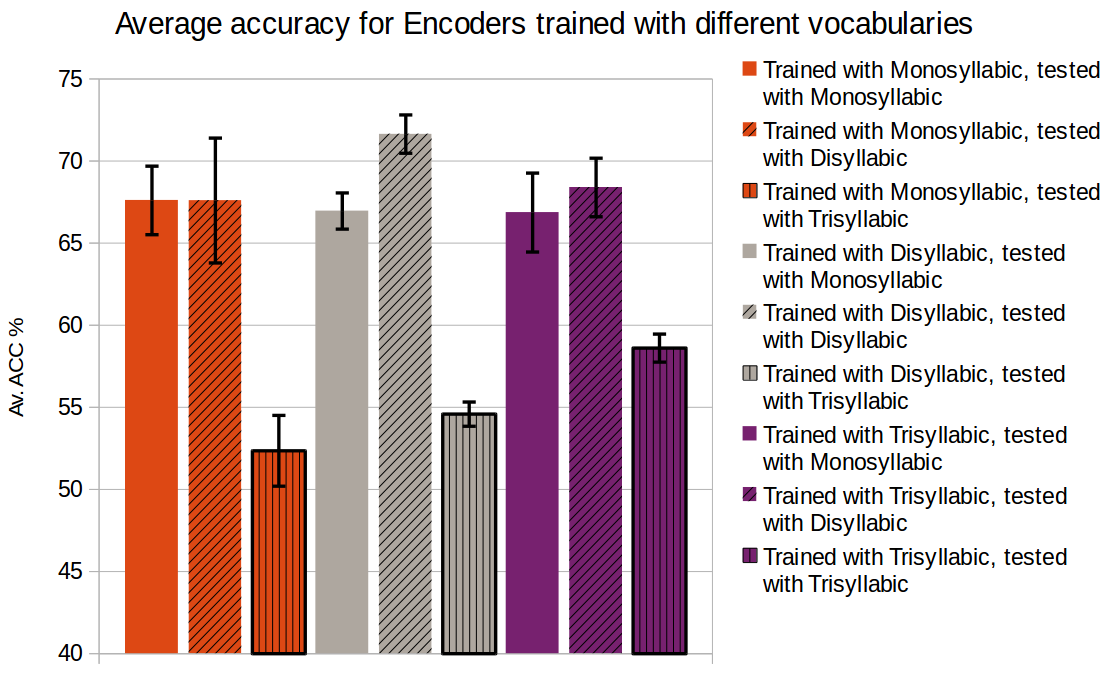
\includegraphics[width=0.9\textwidth]{Encoder_Swept2.png}
    \caption{Desempe\~nos cruzados de clasificación fonética. Las barras de color naranja exhiben los desempe\~nos para \glspl{el} entrenados con palabras monosilábicas, las barras de color gris muestran los desempe\~nos para \glspl{el} entrenados con palabras bisilábicas y finalmente las barras de color violeta muestran desempeños para \glspl{el} entrenados con palabras de tres sílabas. Por otro lado, las barras lisas muestran el desempe\~no de \glspl{el} puestos bajo prueba con palabras monosilábicas, las barras rayadas en diagonal muestran el desempe\~no de \glspl{el} puestos bajo prueba con palabras bisilábicas y las barras rayadas verticalmente muestran el desempe\~no de \glspl{el} puestos bajo prueba con palabras de tres sílabas.}
    \label{fig:E_S2}
\end{figure}


